%In this section, we will explore the causes of the high risk of losses in accessibility for Pacifica, CA.
%Like Danville, Pacifica is at high risk of losses in accessibility, but for different reasons.
%While trip length and bridge vulnerability play a big role in the accessibility risk for Danville, physical conditions contribute significantly to the risk of Pacifica, CA (Figure~\ref{fig:equity_study_area}). \textcolor{red}{TODO: write section}
%In contrast to downtown San Francisco, Pacifica, CA  (Figure~\ref{fig:equity_study_area}) has a high risk of losses in accessibility. We will now explore why. 

%Based on seismic hazard (e.g., Figures~\ref{fig:haz475} and \ref{fig:haz2475}), we might not suspect that Pacifica, CA would be at an elevated risk of accessibility losses across most market segments. In addition, the percentage of pre-earthquake car-based trips is around average for the case study area (88\% versus an average of 85\%). 
%In contrast to most other regions, however, Pacifica is wedged between the Pacific Ocean to the West and the coastal mountains to the East. Indeed, the main access road is California Highway 1, which has various vulnerable bridges included in the case study dataset. There are no viable alternative routes on local roads. Since almost all trips are by car from Pacifica and the average trip length is much longer than the region-wide average (108\% longer), the road issue is particularly serious.

Pacifica is wedged between the Pacific Ocean to the west and the coastal mountains to the east. The main access road is historic California Highway 1, which has a number of older and seismically vulnerable bridges. There are no viable alternative routes to population centers via local roads. Most trips from Pacifica are taken by car (88\%), and the average trip length is 108\% longer than the region-wide average, so the Highway 1 vulnerability is particularly serious.

As a comparison, consider Half Moon Bay, a community about 13 miles to the South (Figure~\ref{fig:pac}). Half Moon Bay has significantly lower expected accessibility losses compared to Pacifica (0.11 $utils$ for a middle income household with fewer cars than workers, versus 0.43 $utils$ in Pacifica). %Yo! Mahalia HMB straddles TAZs 295 and 296. Pacifica is 224.
% For example, for the socio-economic group with middle income households with fewer cars than people who work (Figure~\ref:{fig:scen_acc}{(e)}, the expected accessibility decrease is estimated at xxx $utils$ for Pacifica and only xxx $utils$ for Half Moon Bay. 
While the seismic hazard for the two towns is similar, Half Moon Bay's population is about one third of Pacifica's, so there is less local demand for Highway 1's limited road capacity~\cite{u.s._bureau_of_the_census_united_2010}. Perhaps more importantly, Half Moon Bay has a key alternative to California Highway 1: California Highway 92, which links to the main highways of the peninsula. %The differences in the road topology are illustrated in Figure~\ref{fig:pac}. 
Since Pacifica is unusually reliant on one road with key vulnerabilities, it has an elevated risk for losses in accessibility.
\begin{figure*}[!ht]
    \centering
    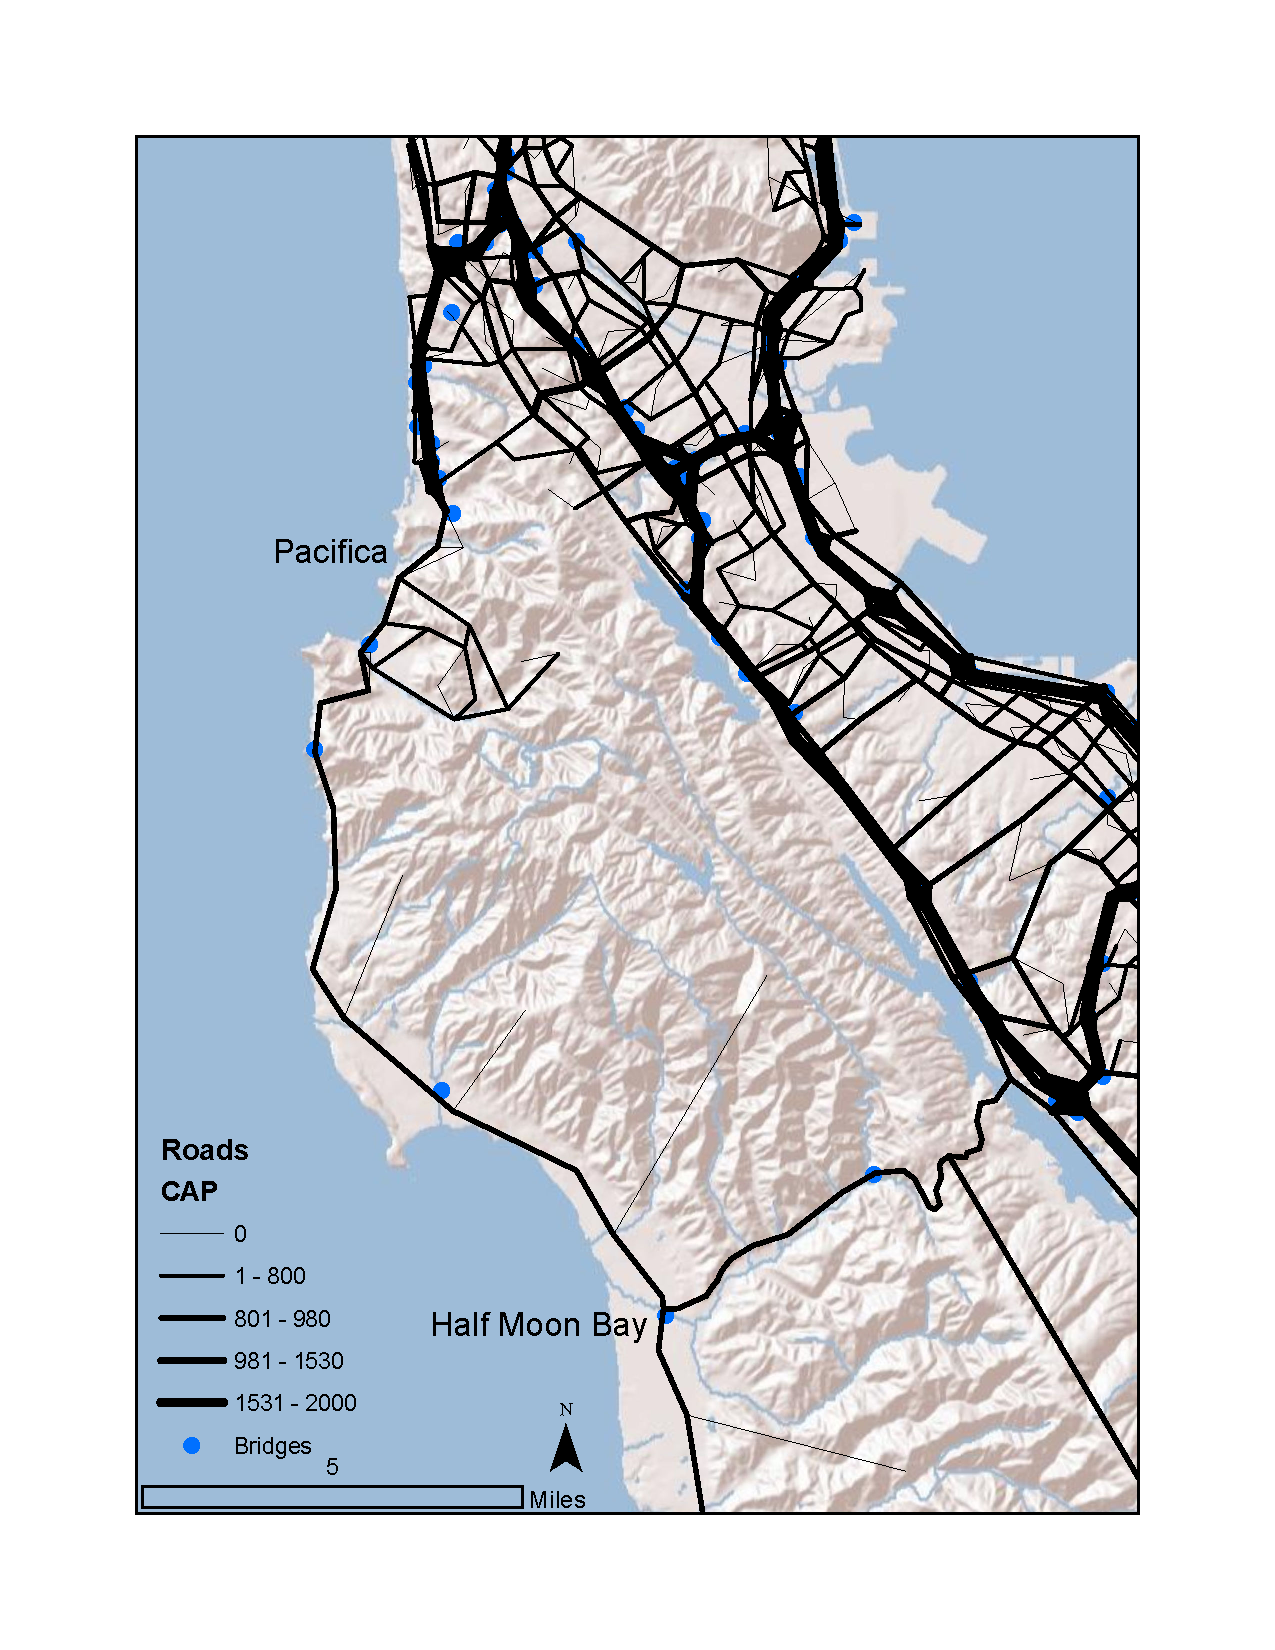
\includegraphics[height=4in]{FIGS/equity_hmb.pdf} 
\caption{Roads providing access from Pacifica and Half Moon Bay.}
\label{fig:pac}
\end{figure*}

%In addition, we see that under normal pre-earthquake conditions, people in Pacifica take much longer trips on average, around 8.57 miles on average, vs. a region-wide average of 6.35 mies

%\begin{figure}
%\centering
%\includegraphics[width=6in]{../FIGS/equity_time_distance_Pacifica.eps} 
%\caption{\textcolor{red}{TODO: add baseline} Trip distributions for trips originating from Pacifica (TAZ 224)  after three earthquake events for a) trip length and b) trip time, as compared to the baseline.}
%\label{fig:time_distance_loss_danville}
%\end{figure}


